\documentclass{beamer}

\usepackage{ucs}
\usepackage[utf8x]{inputenc}
\usepackage{amsmath}
\usepackage{amsfonts}
\usepackage{amssymb}
\usepackage[spanish]{babel}

\usetheme{Copenhagen}
\useoutertheme{infolines}
\setbeamercovered{dynamic}


\title{Introducción al Software Libre}
\author{Entorno de Programación}
\date{2024}
\institute[TUIA - FCEIA]
{Tecnicatura en Inteligencia Artificial \\ Facultad de Ciencias Exactas, Ingeniería y Agrimensura (UNR)}

\begin{document}

\begin{frame}
  \begin{center}
    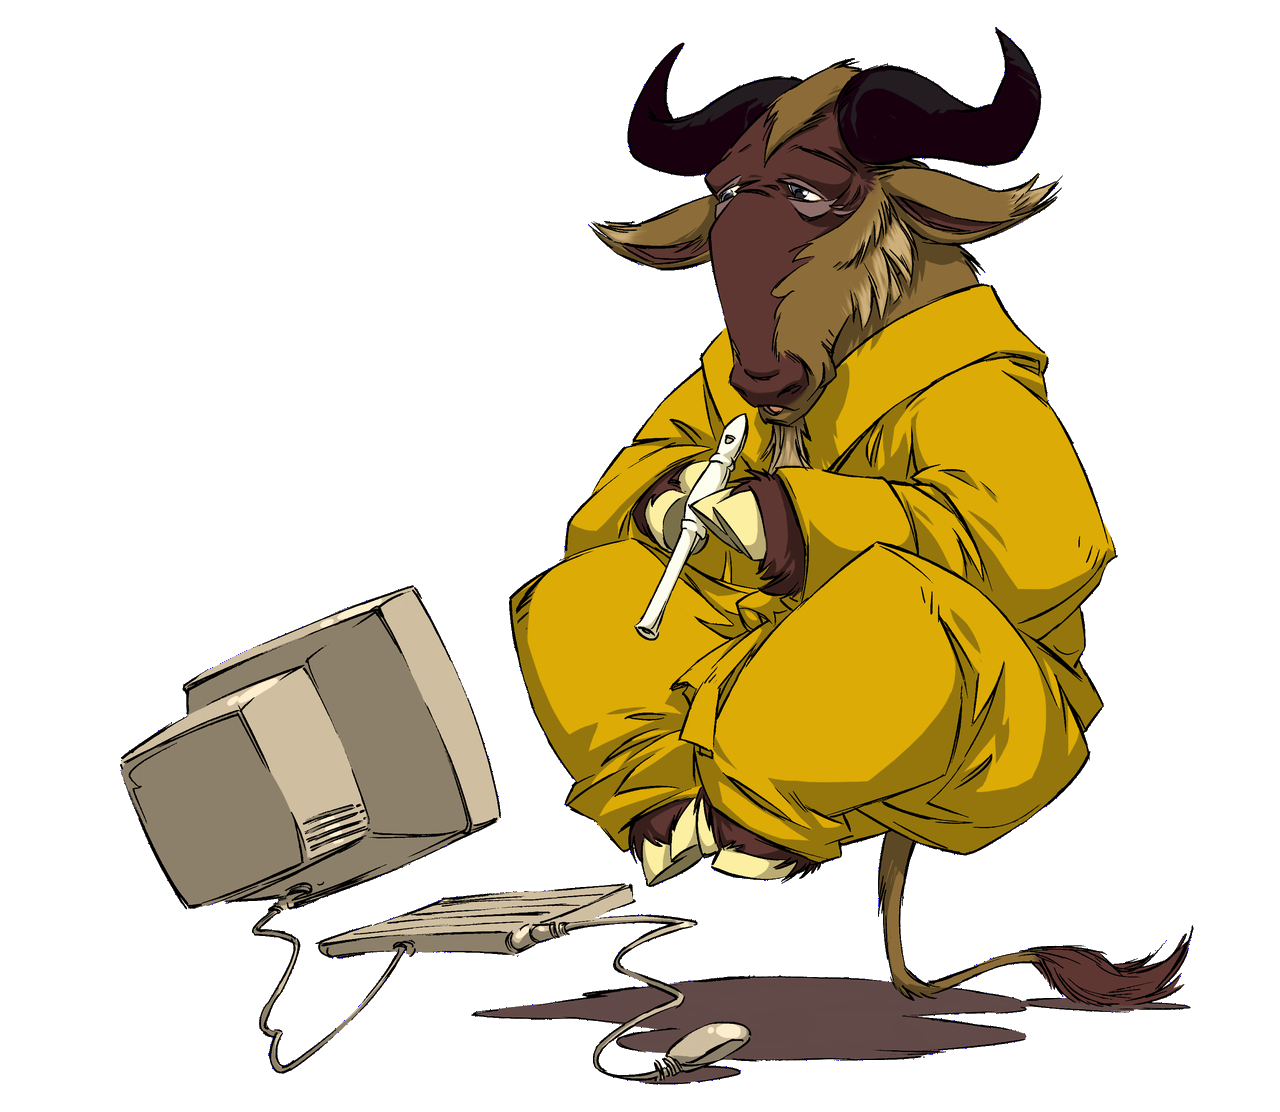
\includegraphics[width=4cm]{pics/meditate.png}
  \end{center} 
  \titlepage
    \begin{center}
      
\includegraphics[width=1cm]{pics/cc-by-sa.png}
    \end{center}
\end{frame}

\begin{frame}
  \frametitle{Fuentes}
  \begin{columns}
    \column{.6\textwidth}
    \centering
    Basado en las dispositivas de Javier Sánchez
    Instituto Español Juan Ramón Jiménez
    Casablanca
    \href{https://www.uco.es/~i02samoj/casablancasl/}{https://www.uco.es/\~{}i02samoj/casablancasl/}
  \end{columns}
\end{frame}

\begin{frame}
  \frametitle{Índice}
  \begin{columns}
    \column{.4\textwidth}
    \begin{flushright}
      
\includegraphics[width=3.5cm]{pics/Official_gnu.pdf}
    \end{flushright}
    \column{.6\textwidth}
    \tableofcontents
  \end{columns}
\end{frame}

\section[Resumen]{}
\AtBeginSection[]{
  \begin{frame}
    \frametitle{Índice}
    \begin{columns}
      \column{.4\textwidth}
      \begin{flushright}
        
\includegraphics[width=3.5cm]{pics/Official_gnu.pdf}
      \end{flushright}
      \column{.6\textwidth}
      \tableofcontents[currentsection]
    \end{columns}
  \end{frame}
}


%  ==============================================================================
% -- INTRODUCCIÓN
%  ==============================================================================

\section{Conceptos básicos}


\begin{frame}{¿Qué es un programa?}
  \begin{block}{Definición}
    Es un conjunto de información lógica que permite a un ordenador cumplir una función.
  \end{block}

  \structure{Componentes}
  \begin{itemize}
  \item Código fuente
  \item Código ejecutable
  \item Datos necesarios: imágenes, sonidos, ficheros de         configuración\ldots
  \item Documentación 
  \end{itemize}

\end{frame}

\begin{frame}
  \begin{exampleblock}{Informática vs. gastronomía}
    \centering 
    \structure{Código fuente} = receta \\ \structure{Código             ejecutable} = tarta
  \end{exampleblock}

  \begin{figure}
    \centering
    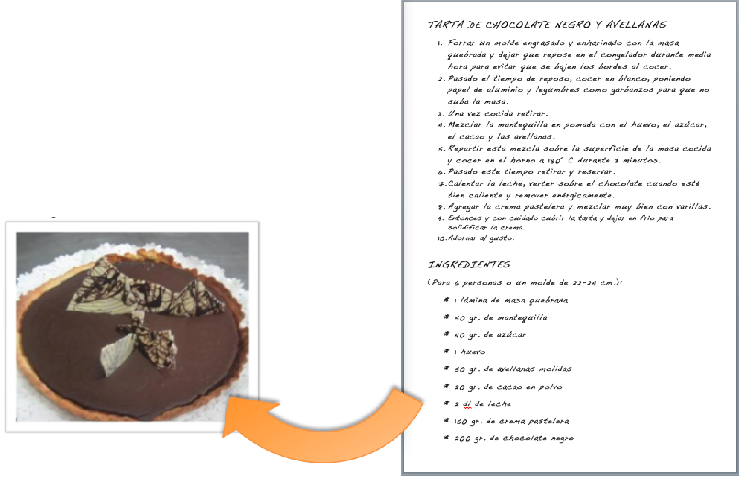
\includegraphics[width=0.7\textwidth]{pics/receta.png}
  \end{figure}
  
\end{frame}


\begin{frame}{¿Qué es el código fuente?}

  \begin{block}{¿Qué es el código fuente?}
    \begin{itemize}
    \item Es la \structure{receta} para hacer un programa de ordenador
    \item Entendible por los humanos 
    \end{itemize}
  \end{block}

  \begin{block}{¿Qué es un fichero ejecutable?}
    \begin{itemize}
    \item Es el \structure{pastel}
    \item Entendible por el ordenador
    \end{itemize}
  \end{block}
\end{frame}


\begin{frame}{¿Qué es la compilación?}

  \begin{block}{¿Qué es la compilación?}
    \begin{itemize}
    \item Es un robot de cocina\ldots
    \item \ldots, un proceso que transforma el \structure{código                 fuente} en un       \structure{fichero ejecutable}
    \item El robot de cocina es el \structure{compilador}
    \end{itemize}
  \end{block}

  \begin{figure}
    \centering
    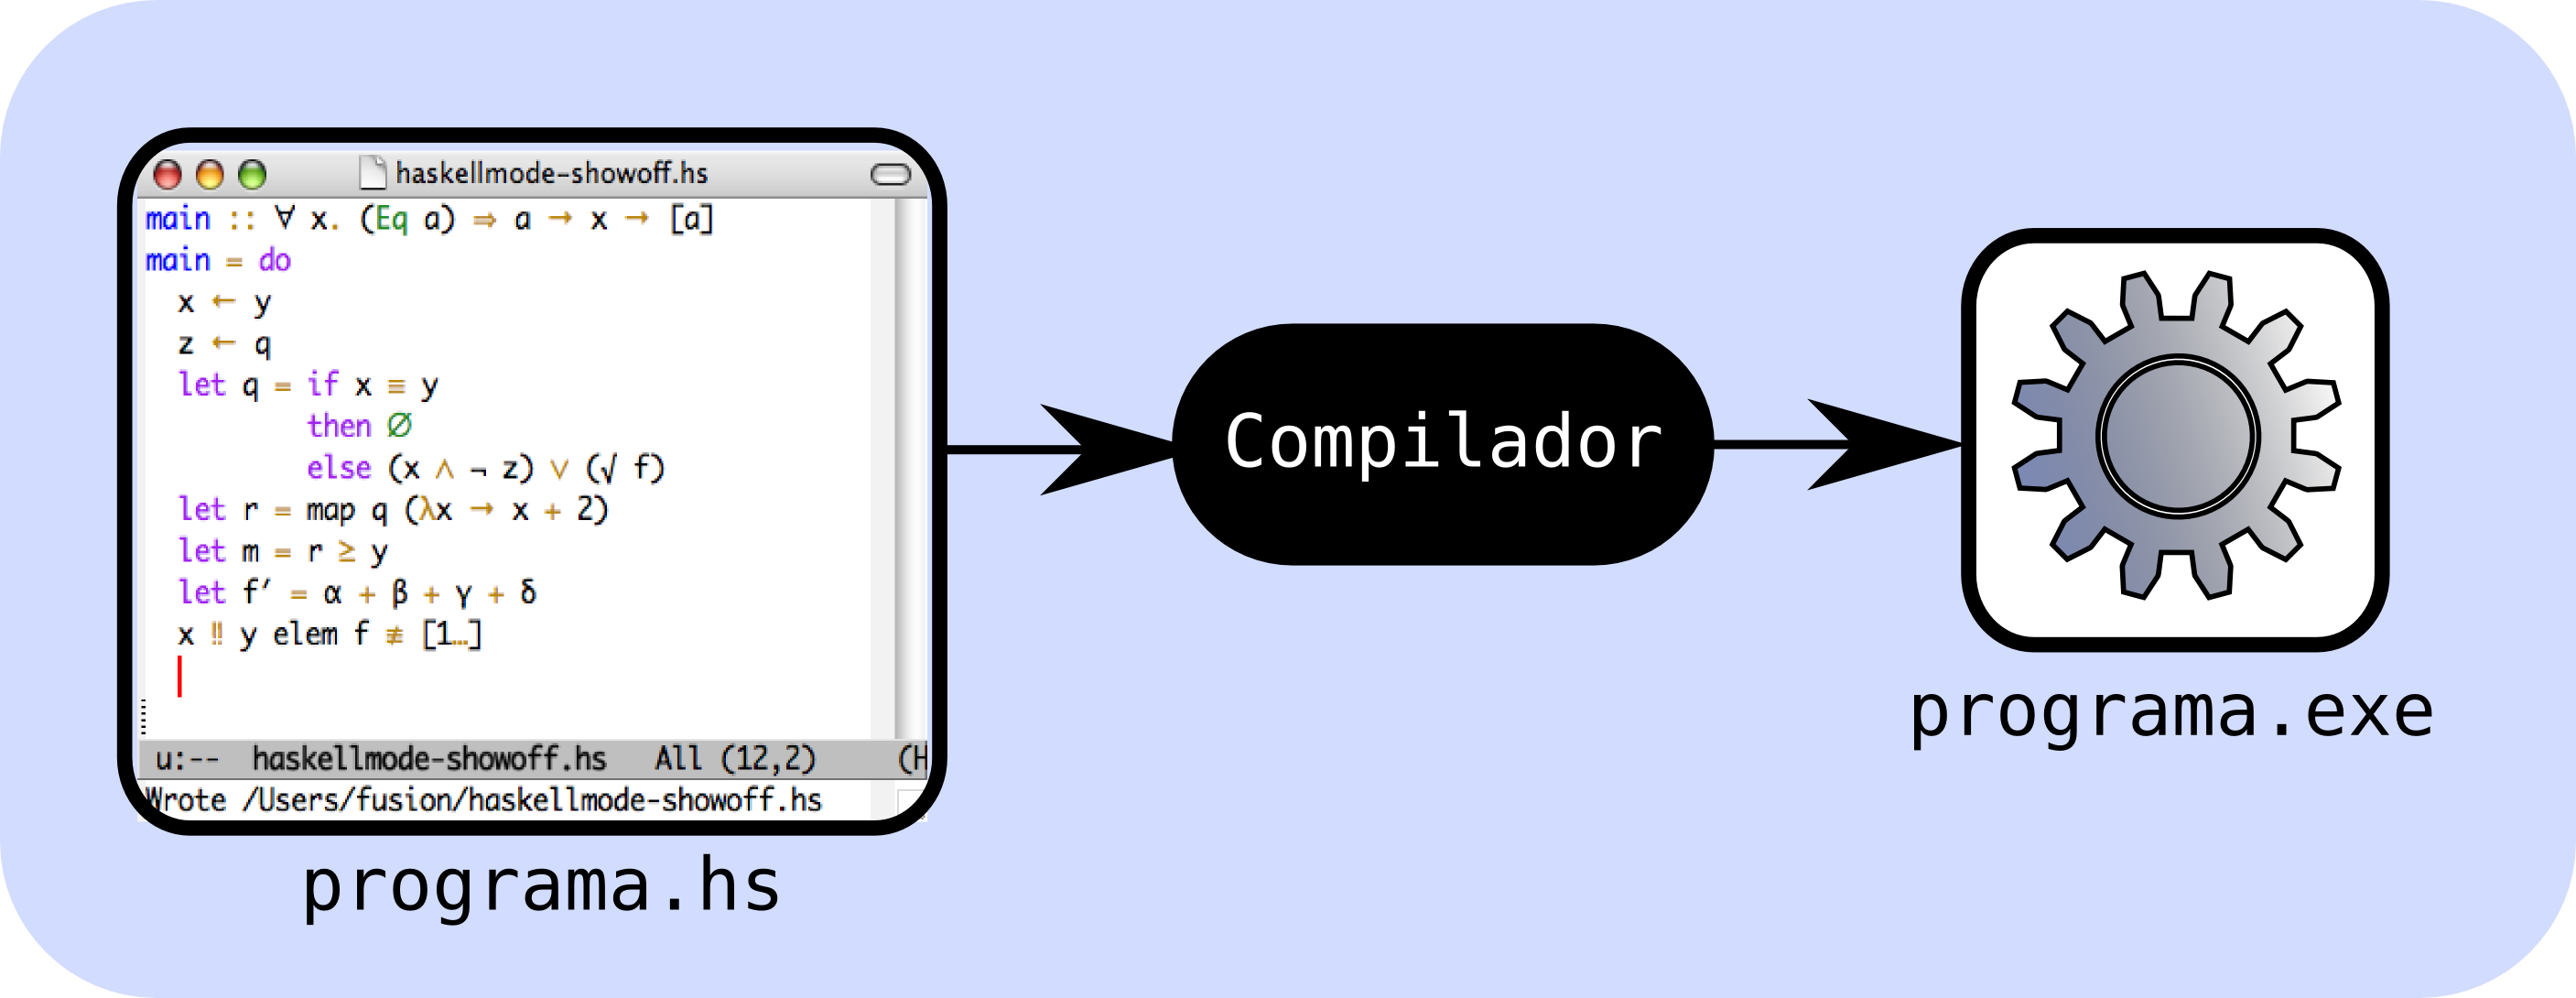
\includegraphics[width=0.7\textwidth]{pics/compilacion.png}
  \end{figure}

\end{frame}

% cárcel del conocimiento
\section{Software privativo vs software libre}
% + Metáfora de la bicicleta: qué cosas prohíbe el software
% + Definición de SL: las 4 libertades
% + SL vírico: Copyleft
% + Licencias

\begin{frame}{El software privativo}
  % Metáfora de la bicicleta: qué cosas prohíbe el software

  \begin{block}{¿Qué es el software privativo?}
    Es software que te obliga a aceptar unas condiciones que restringen la libertad del     usuario.
  \end{block}
  \pause
  \begin{alertblock}{Ejemplos de restricciones de libertad}
    \begin{itemize}
    \item No se vende, sólo obtienes una licencia
    \item No lo puedes compartir
    \item No puedes arreglar el software, ni siquiera el binario
    \item No puedes utilizarlo estás en Cuba, Irán, Sudán, Libia,             Corea del Norte,       Siria\ldots
    \item Das permiso a acceder a información privada, controlar tu             equipo\ldots
    \end{itemize}
    
  \end{alertblock}
\end{frame}

\begin{frame}{El software libre}{Las 4 libertades}
  \begin{columns}
    \column{.7\textwidth}
    \begin{block}{Definición}
      \begin{description}
      \item[Libertad 0] \textbf{usar} el programa, con cualquier                 propósito.
      \item[Libertad 1] \textbf{estudiar} cómo funciona el programa, y                 \textbf{adaptarlo}         a tus necesidades.
      \item[Libertad 2] \textbf{distribuir} copias, con lo que puedes                 ayudar a tu vecino.
      \item[Libertad 3] \textbf{mejorar} el programa y \textbf{hacer                     públicas} las         mejoras a los demás, de modo que toda la                 comunidad se beneficie.
      \end{description}
    \end{block}
    \column{.3\textwidth}
    \begin{figure}
      \begin{center}
        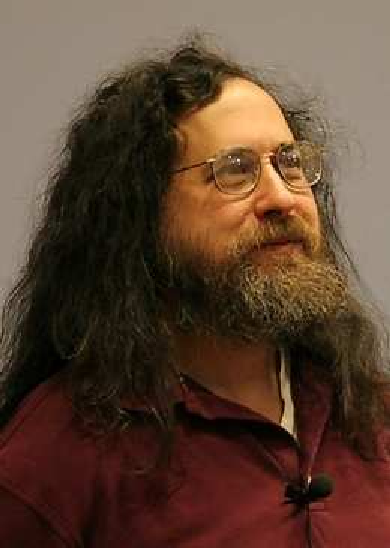
\includegraphics[width=3cm]{pics/richard.pdf}
      \end{center}
      \caption{Richard Stallman}
    \end{figure}
  \end{columns}
\end{frame}

\begin{frame}{El copyleft}{Software libre vírico}

  \begin{block}{}
    \centering ¿Y si alguien toma parte de mi software y lo utiliza de         forma privativa?
  \end{block}
  \pause
  % Notas. Existe software libre sin copyleft
  % La única restricción es que siga siendo libre
  \begin{exampleblock}{copyleft}
    Restricción que se añade al software libre que impide que alguien         distribuya copias o     modificaciones restringiendo las 4 libertades
  \end{exampleblock}

  \begin{figure}
    \centering
    
\includegraphics[width=0.15\textwidth]{pics/copyleft-wetfloo.png}
  \end{figure}
\end{frame}

\begin{frame}{Licencias libres}

  \begin{block}{Garantizar las libertades}
    \begin{itemize}
    \item Se utilizan licencias
    \item Se apoyan en el sistema de \textit{copyrigth} a destruir
    \item Necesidad práctica no ideal
    \end{itemize}
  \end{block}

  
  {\footnotesize
    \begin{columns}[t]
      \column{0.5\textwidth}
      \structure{Con copyleft}:
      \begin{itemize}
      \item GPL: \emph{GNU General Public License}
      \item MPL: \emph{Mozilla Public License}
      \item CC-sa: \emph{Creative Commons-Share Alike}
      \end{itemize}

      \column{0.5\textwidth}
      \structure{Sin copyleft}:
      \begin{itemize}
      \item BSD: \emph{Berkeley Software Distribution}
      \item MIT: \emph{Massachusetts Institute of Technology}
      \item CC: \emph{Creative Commons}
      \end{itemize}
    \end{columns}
  }
\end{frame}

\begin{frame}{Tipos de software}
  \begin{figure}
    \centering
    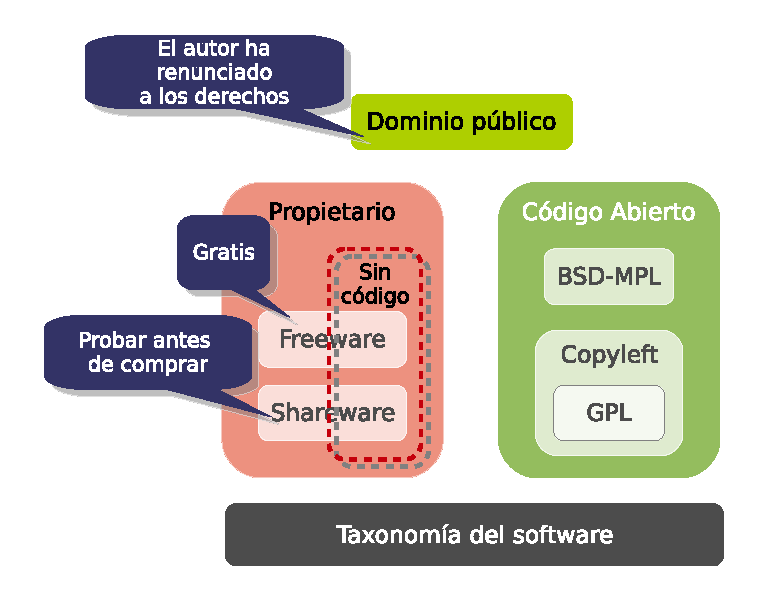
\includegraphics[width=0.8\textwidth]{pics/taxonomia.pdf}
  \end{figure}
\end{frame}


\section{Desarrollo histórico}

% + Contexto histórico
% + Evolución histórica del software (MIT, GNU, Linux...)
% + OpenSource vs. Software libre

\begin{frame}{Los albores de la informática...}

  \structure{Años 60-70}
  \begin{itemize}
  \item Pocas Computadoras:
    \begin{itemize}
    \item Grandes computadoras o \textit{mainframes}
    \item Muy pocos y muy caros
    \end{itemize}

  \item Se desarrolla software artesanal:
    \begin{itemize}
    \item El negocio estaba en el hardware
    \item Poca variedad de software $\Rightarrow$ muy específico
    \item Se dispone del código fuente y los desarrolladores de             software compartían       libremente sus programas unos con otros
    \end{itemize}
  \end{itemize}
\end{frame}


\begin{frame}{...la reacción...}
  \pause
  \structure{Años 80}
  \begin{itemize}
  \item Aparecen las computadoras más modernas y más baratas         $\Rightarrow$ necesidad de     software.
    \begin{figure}
      \centering
      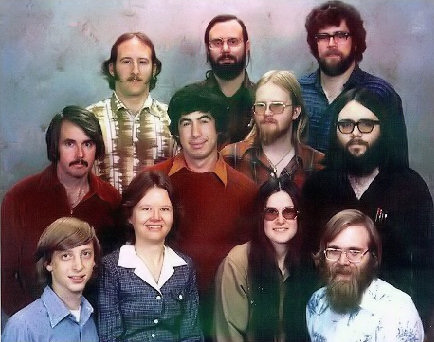
\includegraphics[width=0.3\textwidth]{pics/microsoft1978ew7.jpg}
    \end{figure}
  \pause
  \item El software privativo se hace fuerte:
    \begin{itemize}
    \item Impiden a los usuarios modificar el software
    \item En caso de encontrar un error $\Rightarrow$ comunicar a la             empresa       desarrolladora de ese software
    \end{itemize}
  \end{itemize}
\end{frame}

\begin{frame}{...la revolución...}
  \begin{columns}
    \column{0.6\textwidth}
    \structure{Años 80:} Emerge Richard Stallman
    \begin{itemize}
    \item 1984: comenzó a trabajar en el proyecto GNU.
    \item 1985: funda la Free Software Foundation (FSF). Se introdujeron los conceptos de:
      \begin{itemize}
      \item Free Software \emph{(as in speech)}
      \item Copyleft
      \end{itemize}
    \item Nace el \alert{movimiento social} del software libre.
    \end{itemize}

    \column{0.4\textwidth}
    \begin{figure}
      \centering
      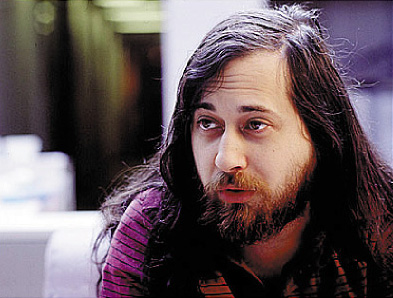
\includegraphics[width=0.6\textwidth]{pics/Richard_Matthew_Stallman.jpeg}
    \end{figure}
    \begin{figure}
      \centering
      
\includegraphics[width=0.6\textwidth]{pics/Official_gnu.pdf}
    \end{figure}
  \end{columns}
\end{frame}



\begin{frame}{...el sistema se completa...}
  \begin{columns}[t]
    \column{0.5\textwidth}
    \structure{Años 90:} en 1991 Linus Torvalds crea el primer núcleo         del sistema     operativo GNU/Linux
    \begin{figure}
      \centering
      
\includegraphics[width=1\textwidth]{pics/gnu-mas-linux.png}
    \end{figure}

    \column{0.5\textwidth}
    \begin{figure}
      \centering
      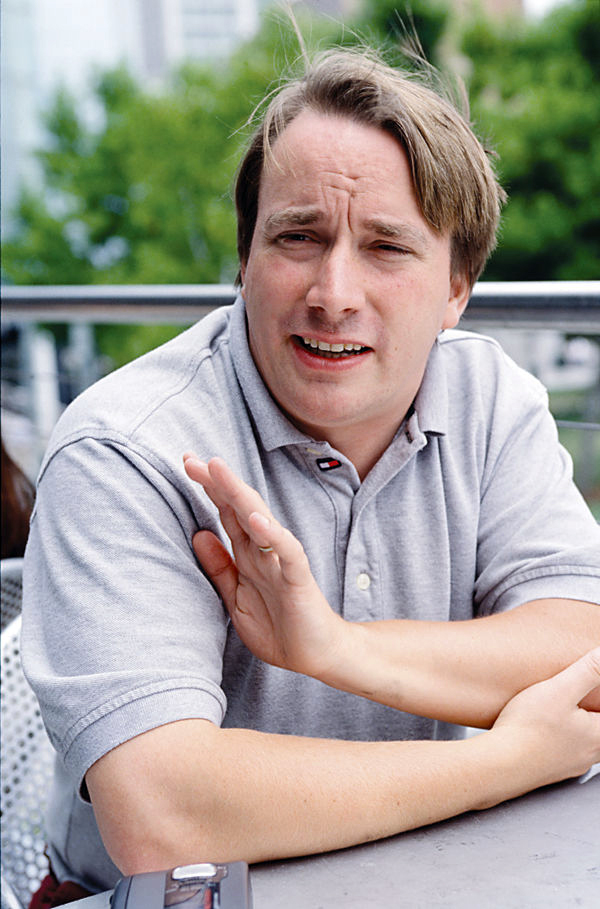
\includegraphics[width=0.6\textwidth]{pics/Linus_Torvalds_talking.jpeg}
    \end{figure}
  \end{columns}
\end{frame}


\begin{frame}{Software libre vs Open Source}
  \begin{columns}
    \column{0.8\textwidth}
    \structure{Años 90:} En 1998 Bruce Perens y Eric S.Raymond fundan         la Open Source     Initiative (OSI). 
    % Es una organización dedicada a la promoción del software de         \structure{fuentes     abiertas}.

    \column{0.2\textwidth}
    \begin{figure}
      \centering
      
\includegraphics[width=0.9\textwidth]{pics/osi-logo.png}
    \end{figure}
  \end{columns}

  \begin{itemize}
  \item Acuñó el término \structure{Open Source}
  \item Evitar la confusión $free = {libre, gratis}$
  \item Aproximar software libre $\leftrightarrow$ empresas
  \item Cambiar el discurso social por el empresarial 
  \item Supuso un cisma con la Free Software Foundation
  \end{itemize}
\end{frame}


\section{El movimiento social}

\begin{frame}{SL e independencia tecnológica}
  \begin{alertblock}{Dependencia tecnológica}
    El \structure{software privativo} (de \textbf{libertad}):
    \begin{itemize}
    \item Centraliza y oculta el conocimiento: monopolios, países,             imperios\ldots
    \item Comportamiento oculto: puertas traseras\ldots
    \item Sujeto a decisiones políticas, económicas\ldots públicas u             ocultas por parte       de empresas y estados
    \end{itemize}
    
  \end{alertblock}

  \pause
  \begin{exampleblock}{Independencia tecnológica}
    El \structure{software libre} (de \textbf{libertad}):
    \begin{itemize}
    \item Descentraliza y libera el conocimiento
    \item El funcionamiento es bien conocido
    \item Permite la independencia y la autogestión
    \end{itemize}
  \end{exampleblock}
\end{frame}


\begin{frame}{SL e independencia tecnológica}
  \begin{exampleblock}{Ejemplos en regiones y estados}
  \end{exampleblock}
  
  \begin{columns}
    \column{0.3\textwidth}
    \begin{figure}
      \centering
      
\includegraphics[width=0.9\textwidth]{pics/huayra-vaca.png}
    \end{figure}

    \pause
    \column{0.7\textwidth}
    \structure{Resultados tangibles}
    \begin{itemize}[<+->]
    \item Huayra GNU/Linux - EDUCAR Sociedad del Estado: \href{https://huayra.educar.gob.ar/}{https://huayra.educar.gob.ar/}
    \item Creación de empresas y cooperativas locales
      % ej.: cooperativa de hackers en Venezuela
    \item Alfabetización digital
      % ej.: Andalucía, Extremadura, Brasil...
    \item Adaptación a idiomas y culturas minoritarias
      % ej.: Linux 192 idiomas vs Windows 90
    \item Independencia de decisiones políticas externas
      % ej.: boikot a la producción de petróleo venezolana
    \item Ahorro en componentes: el hardware caduca cuando se rompe%, no cuando decide el fabricante
    \item Ahorro en licencias 
    \end{itemize}   \end{columns}
\end{frame}


\begin{frame}{SL en la administración pública y la empresa}
  \begin{columns}
    \column{0.3\textwidth}
    \begin{figure}
      \centering
      
\includegraphics[width=0.9\textwidth]{pics/andatuz.png}
    \end{figure}

    \column{0.7\textwidth}
    \structure{Software Libre en la administración}
    \begin{itemize}
    \item Estándares abiertos
    \item Neutralidad tecnológica
    \item Filosofía: lo pagado con dinero público debe ser público
    \end{itemize}
    
    \pause

    \structure{Software Libre en la educación}
    \begin{itemize}
    \item Valor didáctico
    \item No limitante
    \end{itemize}

    \pause
    
    \structure{Software Libre en la empresa}
    \begin{itemize}
    \item Competencia más sana, basada en la cooperación.
    \item \alert{Peligro} 
      \begin{itemize}
      \item Proliferación del término \emph{Open Source}
      \item Uso como publicidad comercial injusta.  
      \end{itemize}
      % Uso de software libre con restricciones para enganchar a los             usuarios con ten
    \end{itemize}
  \end{columns}

\end{frame}

\begin{frame}
  \begin{center}
    \huge
    \setbeamercolor{postit}{fg=black,bg=yellow}
    \alert{¿Preguntas?}\\
    \structure{Muchas gracias por su atención}
  \end{center}
  \begin{center}
    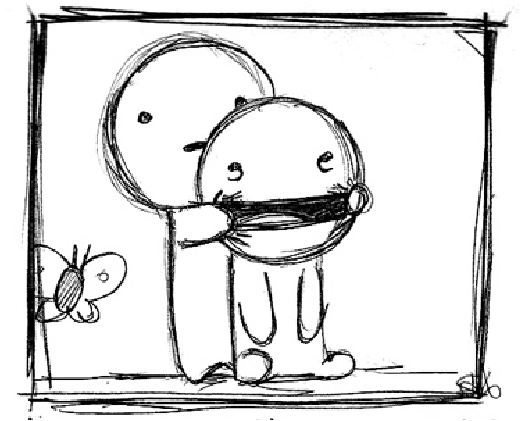
\includegraphics[width=0.5\textwidth]{pics/sonrisa.png}
  \end{center}
\end{frame}

\subsection{Recursos}
\begin{frame}
  \frametitle{Recursos}
  \small
  \begin{thebibliography}{}
  \bibitem[]{psychosynth}
    GNU Project Philosophy
    \newblock Richard Stallman
    \newblock \url{http://www.gnu.org/philosophy/}
    
  \bibitem[]{reactable}
    La Catedral y el Bazaar
    \newblock Eric S. Raymond
    \newblock \url{http://biblioweb.sindominio.net/telematica/catedral.html}


  \bibitem[]{reactable}
    De lo digital a lo analógico
    \newblock Montserrat Boix y Nómada
    \newblock \url{http://www.mujeresenred.net/article.php3?id_article=298}

  \bibitem[]{asd}
    Campañas por el Software Libre
    \newblock Free Software Foundation
    \newblock \url{http://www.fsf.org/campaigns/}

  \end{thebibliography}
\end{frame}

\begin{frame}
  \frametitle{Recursos (II)}
  \small
  \begin{thebibliography}{}

  \bibitem[]{reactable}
    Documentos interesantes
    \newblock Hackmeeting 2008
    \newblock \url{http://sindominio.net/hackmeeting/index.php/Lecturas_recomendadas}

  \bibitem[]{asd}
    Decreto sobre Software Libre y Estándares Abiertos
    \newblock Gobierno de Venezuela
    \newblock \url{http://www.gobiernoenlinea.ve/docMgr/sharedfiles/Decreto3390.pdf}
  \end{thebibliography}
\end{frame}


\end{document}
